\section{The \nfactor~Framework}
\label{sec:overview}

%\subsection{NFActor Framework}

\begin{figure}[!h]
        \centering
        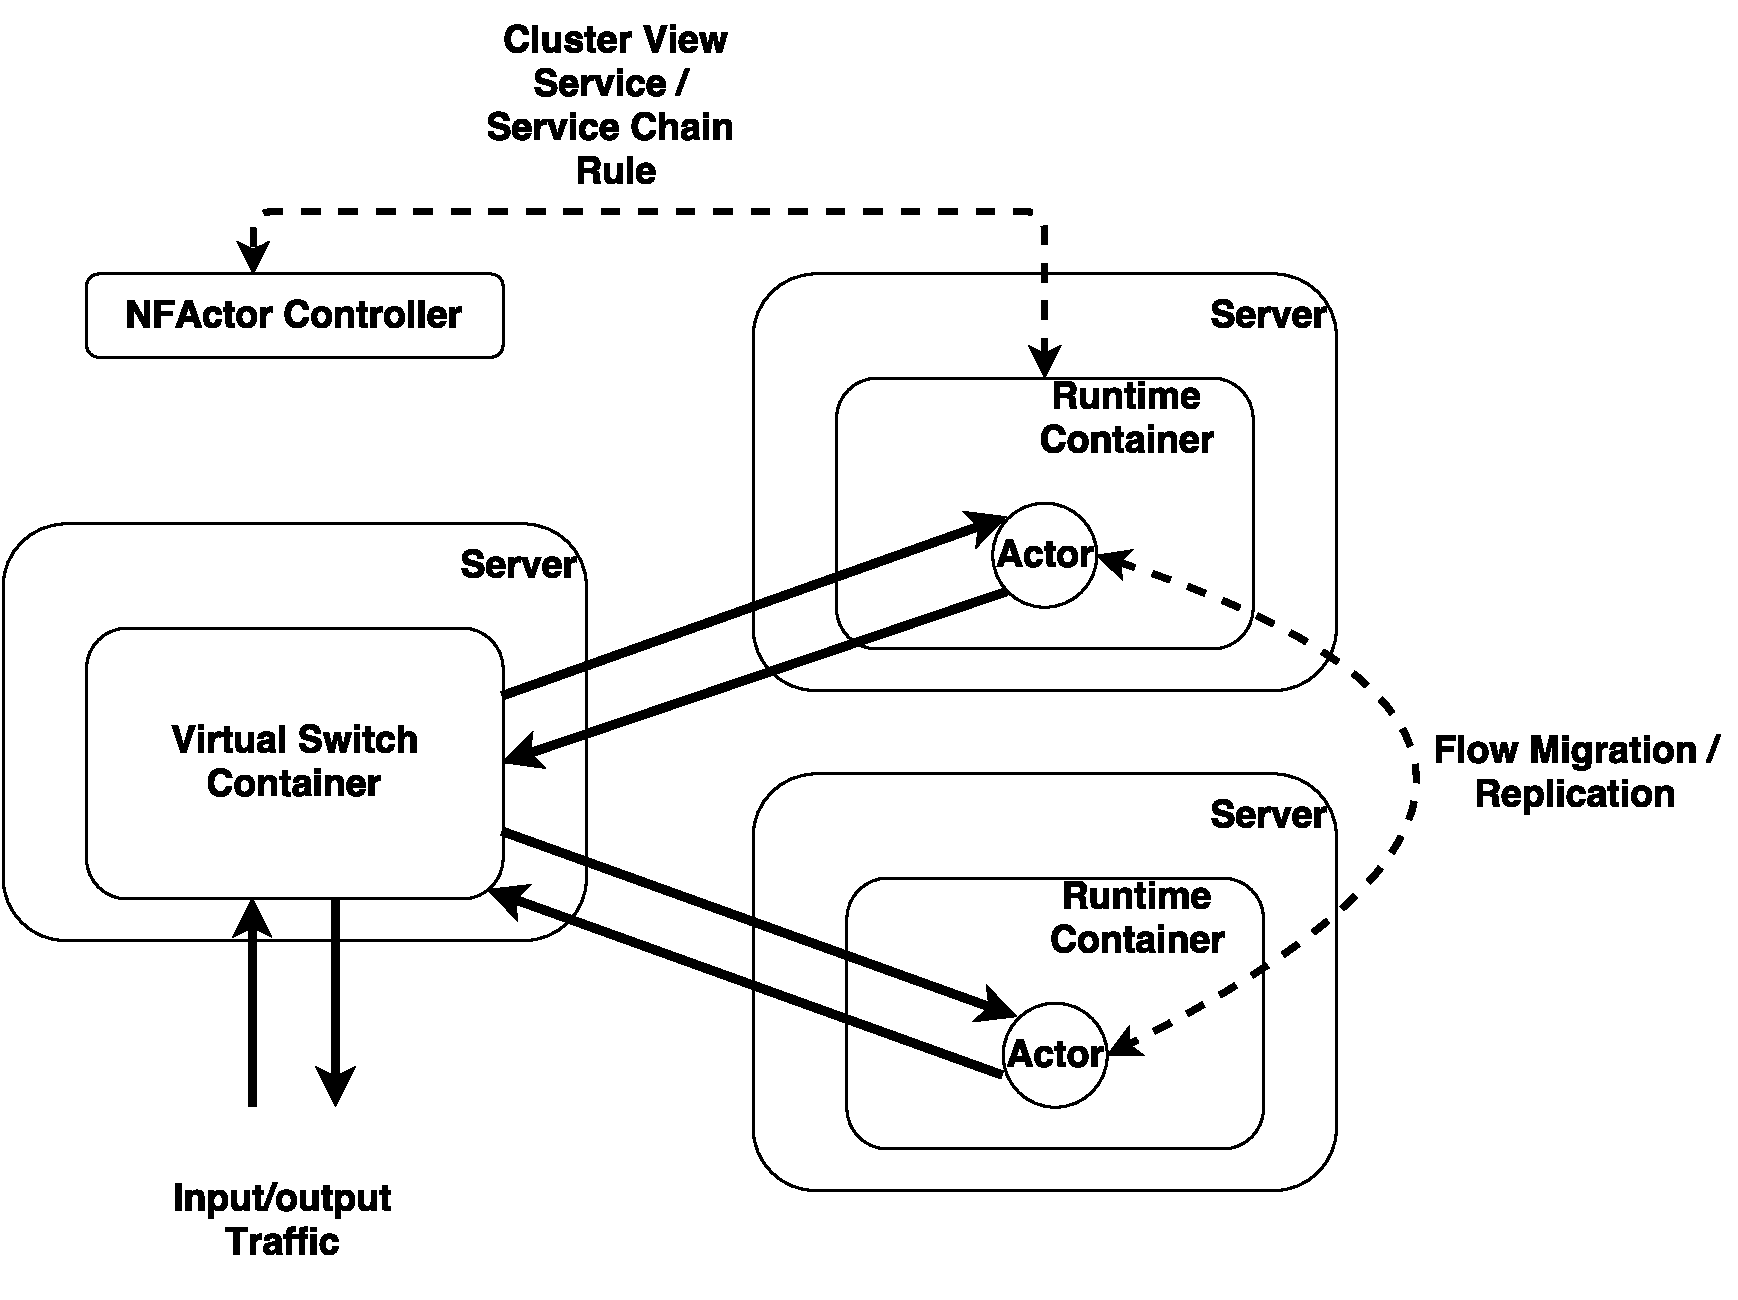
\includegraphics[width=\columnwidth]{figure/NFActor-Overview.pdf}
        \caption{The architecture of \nfactor}
        \label{fig:nfactor-cluster}
\end{figure} 

%\chuan{Fig.~\ref{fig:nfactor-cluster}: as said, remove physical switch which would mislead readers that the system is behind one physical switch}

As illustrated in Fig.~\ref{fig:nfactor-cluster}, %It runs inside a server cluster and 
\nfactor~consists of 3 critical components, a global controller, a global virtual switch and several runtime systems (referred to as {\em runtime} in short). The controller and the virtual switch are logical modules, which can be physically implemented on one or multiple servers or containers according to the workload. In our design, both the virtual switch and runtimes run inside containers, so that they can be quickly rebooted in case of failure, and elastically scaled in case of overload or underload. 

%Frist, talk about the basic work flows of NFActor framework
%The virtual switch acts as a gateway to the NFActor cluster. 
In \nfactor, incoming traffic flows are first sent to the virtual switch, which dispatches them to runtimes in a load-balanced fashion, by querying the load information collected by the global controller. The runtimes host NF service chains, and process the flows. When a runtime system receives a new flow, it constructs a new actor and delegates packet processing of the flow to that actor. The actor queries what NFs the flow should go through by looking for a matching service chain rule. Then the actor loads all the required NF modules to compose the service chain and passes the flow to the NF modules in sequence, before sending the processed flow back to the virtual switch. Finally, the virtual switch sends all the output flows to the respective destinations. 

%Even though NFActor framework has a controller, but the overall operations of NFActor framework, especially those related to flow migration and fault tolerance, do not involve central control. Due to the use of actor model, flow migration and fault tolerance could be executed in a fully distributed fashion. Instead, existing works like \cite{gember2015opennf} relies on controller to initiate flow migration for each flow.

  
%NFActor framework adopts similar cluster design and data plane/control plane
%separation as in E2\cite{palkar2015e2} for efficient management and elastic
%sclaing. Figure \ref{fig:nfactor-cluster} shows a NFActor framework running on a
%server rack. It has a fast data plane (solid arrow line in figure
%\ref{fig:nfactor-cluster}) built over BESS \cite{Han:EECS-2015-155} and a
%control plane (dashed arrow line in figure \ref{fig:nfactor-cluster})
%interconnected through reliable TCP connection for message passing.

%NFActor framework has four componants. The NFActor controller manages the whole
%cluster. The server daemon runs on each physical server inside the cluster, it
%is responsible for setting up the basic server environment and creating/deleting
%containers. There is one NFActor virtual switch and several NFActor runtimes
%in the cluster and all of them run in the containers.

\subsection{Controller}
\label{sec:controller}

Similar with existing work \cite{gember2015opennf, palkar2015e2, sherry2015rollback}, \nfactor~builds a central controller to manage the cluster of virtual switch and runtime systems. Nevertheless, the functionalities provided by this controller are all light-weight ones, including a view service, installing service chain rules and elastic scaling. Due to exploiting the actor model, \nfactor~controller is not directly involved in flow migration and fault tolerance. In contrast, the controllers in existing work are directly involved in supporting failure resilience (if the systems provide the support), by either initiating the flow migration procedure for a flow \cite{gember2015opennf}, or preparing replicas for NF instances \cite{sherry2015rollback}. 

%NFActor controller provides some basic cluster management functionalities,
%including container resource allocation and elastic scaling. But the most
%important functionalities provided by NFActor controller is cluster view
%service and service chain rule.

\textbf{The View Service} identifies and maintains the states and loads of runtimes, using a heartbeat mechanism. Each runtime in \nfactor~regularly sends heartbeat messages to the controller, containing the current load information (\textit{i.e.} CPU usage, memory usage) of the runtime. The controller gathers the information contained in the heartbeat messages into a cluster view list, which records the contact address, state (\textit{running}, \textit{leaving}, \textit{fail}) and load information of all runtimes. The controller broadcasts the cluster view list to each runtime and the virtual switch if there are any state/load changes, so that runtimes and virtual switch have a local copy of this list. The views at different runtime do not have to be consistent because flow migration and fault tolerance protocol perform safety checking by exchanging requests and responses to eliminate the inconsistency. %\chuan{explain that the views at different runtimes do not have to be consistency and the reason}

This view service enables the following: (1) A base for achieving distributed flow migration and fault tolerance. Runtimes can check the received cluster view list to obtain the contact address and load information of other runtimes, and select an appropriate target for flow migration and replication. (2) Facilitating load balancing, as the virtual switch uses the view service to distribute flows to different runtimes. (3) Assisting the controller in making runtime scaling decisions, with the load information it provides.

%A runtime use the view service to retrieve workload
%information, liveness state and contact address of other NFActor runtimes inside
%the cluster. The view service is widely used in cluster
%load-balancing(\cref{sec:vswitch}), flow migration(\cref{sec:fm}) and fault
%tolerance(\cref{sec:ft}).
%It is implemented using a heartbeat mechanism.
%Upon successful creation, the NFActor runtime sends regular heartbeat message to the NFActor
%controller. The heartbeat message contains the instant workload information,
%contact address and an unique ID allocated by the controller. In our current
%implementation, we use container CPU usage as the workload information. The
%controller maintains a cluster view list, which records the latest heartbeat
%message of each NFActor runtime. The view list also records a state field for
%each runtime. The state field has \textit{running}, \textit{leaving} and
%\textit{fail} state. \textit{running} is the default state, \textit{leaving} is
%when the controller decides to shutdown a runtime and send a {\tt leave} message
%to the runtime and \textit{fail} is when no heartbeat message is received within
%a timeout.
%The controller regularly broadcasts the cluster view list to each NFActor runtime and NFActor virtual
%switch, so that NFActor runtimes and NFActor virtual switch all have a local
%copy of the view service. However, the view service is not an always-up-to-date
%service. What NFActor runtime gets from the view service is an instant snapshot of the state
%information. But this does not affect the applicability of the view service. 
  
\textbf{Providing Service Chain Rules.} %In existing works such as \cite{palkar2015e2}, service chains are statically constructed when the NFV system starts up, by creating several NF instances and chaining these instances on the data plane. 
 In \nfactor, the service chain of NFs is dynamically constructed inside the execution context of an actor, depending on the flow it is allocated to process. %In order to correctly retrieve the service chain configuration during dynamic service chain construction, the NFActor framework provides service chain rules. 
 A service chain rule is analogous to an OpenFlow rule \cite{mckeown2008openflow}, installed on the controller to map flows to service chains on the go, to support dynamic service chain construction. It consists of a pattern to match packet headers and a
service chain configuration to specify what NFs the matched packets should go
through in order. A runtime uses service chain rule to determine what service chain
a flow should use. 

In \nfactor, service chain rules are
pre-configured at the controller and pushed to each runtime upon its startup. Pattern matching is implemented as
longest prefix matching over the traditional 5-tuple (source IP,
destination IP, application protocol type, source port and destination port) of a flow,
while the service chain configuration is encoded using a 64-bit integer and every
4 bits of this integer represent a unique NF type.

\textbf{Elastic scaling} is triggered by analyzing the load information
contained in the heartbeat messages. The controller creates new runtime systems when existing runtimes are overloaded (scale-out), or terminates idle runtimes (scale-in). Overload and idling of runtimes are detected according to thresholds on CPU usage.

Once a new runtime system is created, an overloaded runtime can migrate some of its flows to the new runtime until the overload is resolved (add reference). On the other hand, new flows entering \nfactor~tend to choose the new runtime as the target to put replicas (see Sec.~\ref{sec:ft}). When the controller decides to shut down a runtime, it first turns its state into \textit{leaving}. Then this runtime starts migrating all its flows to other runtimes and waits for all of its replicas to expire (Sec.~\ref{sec:ft}). In the meantime, the virtual switch does not route new flows to the \textit{leaving} runtime. The controller shuts down the \textit{leaving} runtime when it becomes completely idle and removes it from the cluster view list. 

\subsection{Virtual Switch}
\label{sec:vswitch}

\nfactor~uses a virtual switch as a gateway for flow dispatching. Previous work either rely on SDN switches \cite{gember2012stratos, gember2015opennf} to route the traffic, or build a customized data-plane for inter-connecting different NF instances \cite{palkar2015e2}. Our virtual switch design results from the following considerations.


\textit{First}, \nfactor~uses uniform runtime systems to process incoming flows and achieves good horizontal scalability. To fully unleash the scalability of \nfactor, we must have a load-balancer to balance the load among different runtimes. Together with the view service, the virtual switch can easily balance the load. \textit{Second}, we can build a customized communication module into the virtual switch, which enables us to design a simple distributed flow migration protocol, bypassing the overhead of communicating with a centralized SDN controller (see Sec.~\ref{sec:fm} for details). \textit{Third}, the virtual switch can be efficiently implemented using an efficient hash table such as cuckoo hashing \cite{pagh2001cuckoo}, and can be implemented in a scalable fashion, so that it will not render a bottleneck in the system. 

The virtual switch maintains a switching hash table, where the key is the hash result of the 5-tuple of a packet,
and the value is the MAC address of the selected runtime for handling the flow. Whenever the first packet of a new flow arrives, the virtual switch
selects a runtime in the \textit{running} state from the view service using
a round-rubin algorithm. We choose a simple round-rubin algorithm because the virtual switch must run very fast and round-rubin algorithm introduces the smallest amount of overhead while providing satisfactory performance. %\chuan{shouldn't it be based on load info of the runtimes, i.e., higher probability to dispatch to one runtime with lower load?}
, adds a key-value pair in the hash table, and forwards the packet to the selected runtime by replacing its destination MAC address by the MAC address of the runtime. Later packets from the same flow still needs to check the hash table. However, this overhead is greatly reduced by using a fast hash table like Cuckoo hash table \cite{zhou2013scalable}. %\chuan{explain whether later packets in the same flow still need to check the hash table}

\subsection{Runtime}
\label{sec:runtime}

\begin{figure}[!h]
        \centering
        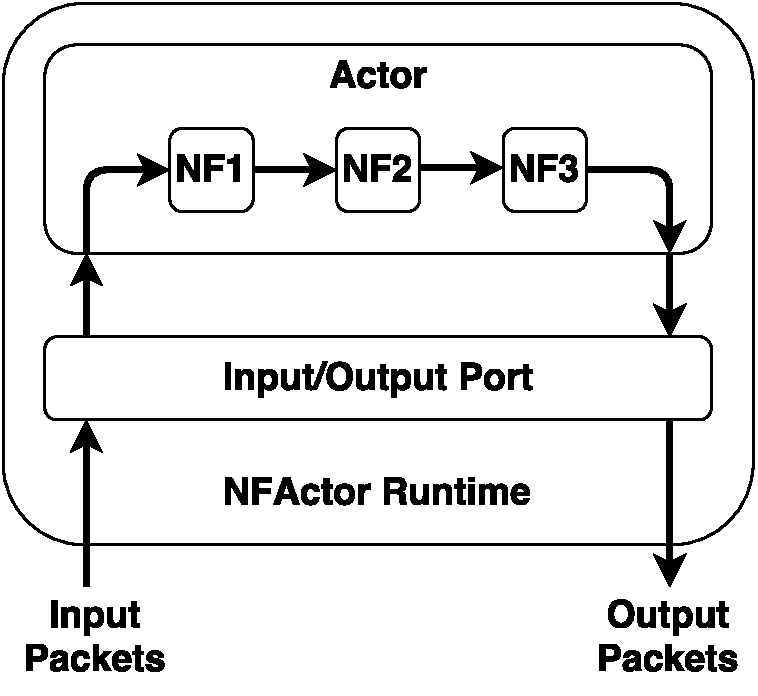
\includegraphics[width=0.6\columnwidth]{figure/NFActor-Runtime.pdf}
        \caption{The architecture of a \nfactor~runtime system}
        \label{fig:nfactor-runtime}
\end{figure} 

%\chuan{Fig.~\ref{fig:nfactor-runtime}: revise the figure as we discussed before, e.g., removing the flow classifier from the output path, putting NFs into the actor, etc.; explain in a following paragraph what the flow classifier is for}
%We choose to design a uniform runtime system for NFActor framework as the basic flow processor. It's over-all architecture is shown in Fig.~\ref{fig:nfactor-runtime}. On contrary to NFActor framework, 

The concept of a uniform runtime system (Fig.~\ref{fig:nfactor-runtime}), as a basic flow processing and scaling unit in \nfactor, does not appear in most existing work \cite{bremler2015openbox, gember2012stratos, palkar2015e2}. In existing NFV systems, the basic flow processing and scaling unit is an NF instance, which is a virtual machine or container hosting an instance of a NF. % and the NF instances are chained on the data-plane. % The flows must go through these NF instances in sequence. 
 The primary reason that we design a uniform runtime is to enable NF modules to achieve resilience automatically in the \nfactor~framework without manual intervention. As the uniform runtime system provides a network transparent abstraction for actors to communicate and exchange messages that are crucial to migration and replication. % \chuan{clarify why uniform runtime leads to automatic resilience}. % we want NF softwares written using NFActor framework to achieve resilience automatically without manual intervention.
  Especially, in a runtime system, we adopt the simple yet powerful design to create a micro execution context for each flow, and encapsulate processing functions of the flow over its entire service chain inside the micro execution context. Then we can enable resilience on the basis of each micro execution context (Sec.~\ref{sec:ft}). To be able to process multiple flows, the runtime system should be capable of handling multiple micro execution contexts concurrently. This is handled using a similar hash-table based flow classifier as mentioned in Sec. \ref{sec:vswitch}.

In \nfactor, we exploit the actor programming model to implement the micro execution context. Each micro execution context is an actor. Flow processing by NFs in the service chain, flow migration and replication functionalities are all implemented as message handlers of the actor. The runtime system provides the basic runtime environment for all the actors it has created. In particular, it creates a new actor when a new flow is sent to it. The actor looks for a matching service chain rule for the flow and loads the corresponding NF modules specified in the rule. Then the actor processes the flow by passing the packet through each NF module in sequence, as well as performs flow migration and states replication in response to certain messages (Sec.~\ref{sec:ft} and Sec.~\ref{sec:fm}). 

Besides built-in resilience, additional benefits are brought by our uniform runtime system design. \textit{First}, it simplifies service chain management. In previous work such as \cite{palkar2015e2}, the controller must create several different service chains on the data-plane. %, each consisting of different kinds of NF instances. 
 In \nfactor, service chains are dynamically created inside each runtime in a very lightweight fashion without directly involving the controller. \textit{Next}, with the help of a load-balancing virtual switch, our framework can easily scale out by adding more runtimes. In previous work \cite{palkar2015e2}, scaling-out involves modifying data-plane network paths, which is not trivial.

Each runtime can host one or multiple actors, depending on its resource availability and performance isolation requirements. In case of a multi-tenant NFV system, we can run actors processing flows of the same tenant on the same runtime, but those of different tenants on different runtimes, for better security and isolation. When multiple actors are running on the same runtime, the actors are scheduled to run on a worker thread whenever a message is sent to the actor's mailbox. The actor %\chuan{discuss how the actors are scheduled/resources are allocated to the actors}. 
In addition, our design of the NF modules in the following section will show that passing packets to a NF for processing in an actor is essentially just a function call; only one copy of each NF module software needs to be loaded in a runtime, while multiple actors hosting service chains involving the NF can use it. The actor itself is a very lightweight one as millions of actors could be spawned in seconds \cite{chs-rapc-16}. %\chuan{emphasize more of the lightweightedness of the actor model.} 
To further reduce overhead of loading NF modules in the runtimes, the virtual switch can direct flows requiring a similar set of NFs to the same runtimes.


%NFActor framework chooses to provide a uniform runtime system as shown in figure ~\ref{fig:nfactor-runtime}.  This is 

%NFActor runtime is dynamically created by the controller during system
%initialization and elastic scaling. Each NFActor runtime is created with 3
%ports, one for receiving input data-plane packets, one for sending output
%data-plane packets and one for transmitting control-plane messages. 

%NFActor
%runtime joins the cluster upon successful creation. It keeps sending regular
%heartbeat message to the controller to maintain its \textit{running} state. If
%the workload of a runtime is small, the controller may send a {\tt leave}
%message to the runtime, asking the runtime to leave the cluster. The runtime
%migrate (\cref{sec:fm}) all of its flows to other NFActor runtimes with
%\textit{running} state and wait for all the flow state replicas (\cref{sec:ft})
%to expire. Then the runtime responds the controller with a {\tt ok} response and
%the controller will shutdown the runtime.

%The NFActor runtime handles the actor creation and packet processing. It's
%internal architecture is shown in figure \ref{fig:nfactor-runtime}. The input
%path of the NFActor runtime starts by receiving a batch of packets using a polling
%thread\cite{dpdk}. Then these input packets are sent to a flow classifier.
%The flow classifier is similar to the switching hash table in
%\cref{sec:vswitch}, except that the value in the flow classifier is the unique
%actor id assigned by the NFActor runtime. Flow classifier tries to send the
%packet to a created actor. If there's no actor for handling the packet, a new actor is
%created. The actor processes the packet by passsing the packet along the service chain.
%On the output path, the actor first sends the packet to the flow classifier to
%record a mapping for the reverse flow. Then the packet are sent out to the
%virtual switch from the output port.

%Using NFActor framework inevitably adds more overhead for packet processing,
%because of the existance of the flow classifier and actor processing.
%But the with the help of fast hash table design like cuckoo hashing
%\cite{zhou2013scalable, pagh2001cuckoo}, the overhead for flow classifier could
%be greatly mitigated. The overhead of using actor could also be optimized by
%e-designing the actor scheduler. We leave these optimizations to future work on
%NFActor.

\subsection{An API for Creating NF Module}

\begin{figure}[!t]
	\begin{subfigure}[b]{\columnwidth}
		\centering
 	 	\lstset{language=C++, numbers=left, showspaces=false,
    		showstringspaces=false, tabsize=2, breaklines=true,
    		xleftmargin=5.0ex, basicstyle=\scriptsize,
		}

		\begin{lstlisting}
class flow_state{
};

class network_function{
public:
  virtual void init() = 0;
  virtual flow_state* allocate_flow_state() = 0;
  virtual bool process_packet(rte_mbuf* pkt, flow_state* fs) = 0;
  virtual serialized_obj serialize_flow_state(flow_state* fs) = 0;
  virtual flow_state* deserialize_flow_state(serialized_obj* obj) = 0;
};
		\end{lstlisting}
		\caption{An API for creating new NF module.}
		\label{fig:api}
    \end{subfigure}\hfill
	\begin{subfigure}[b]{\columnwidth}
		\centering
 	 	\lstset{language=C++, numbers=left, showspaces=false,
    		showstringspaces=false, tabsize=2, breaklines=true,
    		xleftmargin=5.0ex, basicstyle=\scriptsize,
		}

		\begin{lstlisting}
class state : public flow_state{
public:
  state():pkt_counter(0){};
  serialized_obj serialize() override{
    return serialized_obj(pkt_counter);
  }
  int pkt_counter;
};

class pkt_counter : public network_function{
public:
  void init() {};
  flow_state* allocate_flow_state() override{
    return new state();
  }
  bool process_packet(rte_mbuf* pkt, flow_state* fs) override{
    state* s = dynamic_cast<state*>(fs);
    if(!s){
      rte_pktmbuf_free(pkt);
      return false;
    }
    s->pkt_counter+=1;
    return true;
  }
};
		\end{lstlisting}
		\caption{A example NF module created using the API.}\label{fig:example}
	\end{subfigure}
\caption{The API and implementation of an example NF module.}
\label{fig:base-class}
\end{figure}
%\chuan{Fig.~\ref{fig:api}: replace the simple NF by a more realistic one, e.g., firewall or IDS or else}

With the micro execution context enabled by the runtime and the actor model, we need one last step towards achieving built-in resilience, which is %providing a rule
 to separate important NF states from the core processing logic of the NF module. With this separation, the actor can retrieve and serialize NF states for transmission whenever needed, without interfering with processing logic execution of the NF module. In \nfactor, we achieve this separation by designing an API for implementing new NF modules in the actor model. 

Fig.~\ref{fig:api} illustrates this API. To implement a new NF class, programmer must use {\tt network\_function} as the base class and implement all 5 virtual methods. The {\tt init} method is used by the runtime to initialize the NF module upon startup. When a new actor is created to handle a new flow, it first calls the {\tt allocate\_flow\_state} method to create a local flow state object. Whenever the actor receives a new packet, the actor passes the received packet (represented as {\tt rte\_mbuf}) and the flow state object to the {\tt process\_packet} method for NF processing. The return value of {\tt allocate\_flow\_state} indicates whether the packet should continue to be processed on the service chain. During flow migration and replication, the actor uses the last 2 methods to serialize flow state object for transmission and de-serialize {\tt serialized\_obj} to recover the flow states. 

This API design turns a NF module into a state machine: %. From the perspective of an actor, 
NF processing is to feed the current event (input packet) and current state (flow state) into the state machine (NF module), generating a new state (updated flow state) and a new action (processed packet). This API design enforces the separation between flow states and processing logic of the NF, so that the actor can easily and correctly retrieve flow state for transmission during flow migration and replication.

%Figure \ref{fig:api} shows the base class used to create new NF module. To
%create a new NF module, the programmer should define a new NF module class by
%deriving from {\tt network\_function} and a corresponding flow state class
%by deriving from {\tt flow\_state}. The runtime initialize all the NF
%modules by calling their {\tt init} method upon start up. When a new actor is
%created, it stores pointers to all the NF modules as indicated in the service
%chain rule (\cref{sec:controller}). Then the actor asks each NF module on the
%service chain to allocate a per-actor flow state object, by calling {\tt
%allocate\_flow\_state} method. When the actor receives a new packet (represented
%as a {\tt rte\_mbuf*}, the default packet representation in DPDK\cite{dpdk}), it calls {\tt process\_packet} method
%of the NF module to process the packet. The return value of {\tt
%process\_packet} indicates whether the NF module has finished processing the
%packet. If the return value is true, the NF module finishes processing the
%packet and the packet could be passed to the next NF module on the service
%chain, or be sent out from the output port. If the return value is false, the
%packet is temporarily buffered in the flow state object, waiting for a
%asynchrounous notification to resume its processing on the service chain. This
%could be used to implement shared queues as in Click modluar router \cite{kohler2000click}.

%We use a simple example to demonstrate how to create a new NF module. In figure
%\ref{fig:base-class}, we define a simpile NF module class {\tt pkt\_counter}, it
%counts the number of flow packets that it receives. We first define a {\tt
%state} class which contains a state variable {\tt counter}. Then we define a
%{\tt pkt\_counter} class and implement required virtual functions. When the actor is created,
%a new flow state object {\tt state} is created. When the actor receives an input
%packet, it calls {\tt process\_packet} function to add the {\tt fs.counter} by 1. 



